\documentclass[12pt]{ctexbook}

\usepackage{amsmath,amssymb}
\usepackage{graphicx}
\usepackage{booktabs}
\usepackage{hyperref}
\usepackage{geometry}
\geometry{a4paper,margin=2.5cm}

\title{天津财经大学博士毕业论文示例题目}
\author{张三}
\date{2026年5月}

\begin{document}
\maketitle

\frontmatter
\chapter*{摘要}
这是一个公开示例文档，用于测试 LaTeX 到 DOCX 的转换流程。本文中的人物、编号、研究内容和数据均为虚构占位内容。

\textbf{关键词：} 数字经济；产业升级；实证研究

\chapter*{Abstract}
This public sample demonstrates a LaTeX-to-DOCX workflow. Names, IDs, research content, and data in this document are placeholders.

\textbf{Keywords:} digital economy; industrial upgrading; empirical research

\tableofcontents

\mainmatter
\chapter{绪论}
\section{研究背景}
这里是公开占位正文。你可以在自己的论文项目中替换为真实内容，但不要把真实论文正文提交到公开仓库。

\section{研究方法}
本文展示普通段落、脚注\footnote{这是公开示例脚注。}、公式、图和表的基本转换。

\begin{equation}
Y_{it}=\alpha+\beta X_{it}+\gamma Z_{it}+\mu_i+\lambda_t+\varepsilon_{it}
\end{equation}

\begin{figure}[htbp]
  \centering
  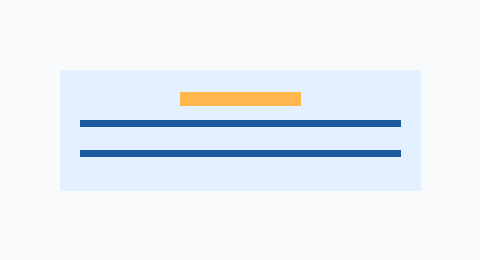
\includegraphics[width=0.6\textwidth]{figures/example.png}
  \caption{公开占位示意图}
  \label{fig:example}
\end{figure}

\begin{table}[htbp]
\centering
\caption{公开占位表格}
\label{tab:example}
\begin{tabular}{lcc}
\toprule
变量 & 均值 & 标准差 \\
\midrule
$x$ & 1.23 & 0.45 \\
$y$ & 2.34 & 0.67 \\
\bottomrule
\end{tabular}
\end{table}

如图~\ref{fig:example} 和表~\ref{tab:example} 所示，这些内容只用于模板测试。

\chapter{文献综述}
这里放置公开占位文献综述内容。引用示例可以在后续接入 BibTeX 或 CSL 工作流。

\chapter{结论}
本样例说明了如何组织一个最小可运行的 LaTeX 论文输入，并通过 Pandoc 及后处理脚本转换为 DOCX。

\backmatter
\chapter*{致谢}
感谢开源工具社区。本致谢为公开占位文本。

\end{document}
